%=================================================================
\section{Introduction}\label{sec-intro}

% Test citation~\cite{BL12J01}. 
% \begin{JournalOnly}
% and~\citep{BJL11J01} or~\citet{BJL11J01}.
% \end{JournalOnly}
     Summary:Classify the sentiment of sentences from the Rotten Tomatoes
    dataset\\
    Every years,there are many movies appear on the screen.We can read com-
    ments to know a movie is good or not\\
    Movie Reviews come from varying people.Some may say the positive re-
    views,others may say the negative comments of the movies.We can classify
    a movie by it’s comments.But the reviews is a large dataset,people can’t read
    every comments.\\
    Here it is,we can use computer to classify the dataset.
    According to the reviews to distinguish sentiments.
% \todo[fancyline]{Testing.}
% % and this is for~\cref{sec-conclusions}.
% \todo[noline]{A note with no line back to the text.}%
% \gangli{This is comment from Gang.}
% \qwu{Response from QW}

% Number:
% \num{123}.
% \numlist{10;30;50;70},
% \numrange{10}{30},
% \SIlist{10;30;45}{\metre},
% and
% \SI{10}{\percent}

% \missingfigure[figcolor=white]{Testing figcolor}
% 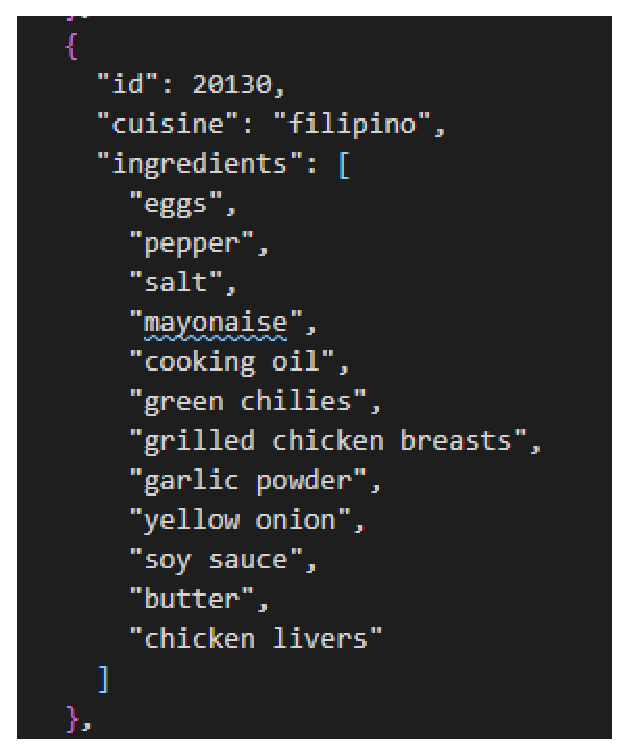
\includegraphics[width=0.4\textwidth]{train.eps}

\includegraphics[width=0.45\textwidth]{D://Code//Kaggle-test//Data//header.png}

% \begin{ConferenceOnly}
% We have \SI{10}{\hertz},
% \si{\kilogram\metre\per\second},
% the range: \SIrange{10}{100}{\hertz}.
% $\nicefrac[]{1}{2}$.

% \missingfigure{Make a sketch of the structure of a trebuchet.}
% \end{ConferenceOnly}
% This is test data\\
% \includegraphics[width=0.4\textwidth]{test-data.png}

% For~\cref{eq:test},
% as shown below:

% \begin{equation}\label{eq:test}
% a = b \times \sqrt{ab}
% \end{equation}
% \begin{minted}{Python}
% 	employees = []
% 	for id in employee_ids:
% 	    employee = fetch_employee(id)
% 	if employee:
% 	    employees.append(employee)
% \end{minted}
% \blindmathpaper

\section{Data} \label{sec-preliminaries}

This event provides two data sets that can be used: train.tsv  test.tsv\\
\textbf{train.tsv}: contains the phrases and their associated sentiment labels.
    We have additionally provided a SentenceId so that you can track which
    phrases belong to a single sentence.\\
\textbf{test.tsv}:contains just phrases. You must assign a sentiment label to eachphrase.

% \gliMarker  %TODO: GLi Here


\section{Data Processing} \label{sec-method}
\begin{itemize}
  \item
  Read Data \\
  \begin{itemize}
  \item
  Read train.tsv
  \item
  Read test.tsv
  \end{itemize}
  \item
  Processing Model:Bag-of-words model (BoW model)\\
  \begin{itemize}
    \item 
    BoW early in Natural Language Processing and Information Retrieval 
    This model ignored the grammar and word order elements such as text, 
    just as it is a collection of several words, the emergence of each
     word in the document are independent of each otherBoW to use an 
     unordered list of words to express a text or a document.
  \end{itemize}
   \begin{itemize}
    \item
    CountVectorizer is a characteristic class of common numerical calculation,
    Is a text feature extraction method.For each training text, it only considers 
    each of these words in the frequency of the training in the text.
    CountVectorizer Converts text of the words in the word frequency matrix.
    It does this by fit_transform function calculating the number of occurrences of all words.
    \end{itemize}
  \begin{itemize}
    \item  TF-IDF model\\
    TF - IDF (term frequency, inverse document frequency) is a kind of commonly 
    used for information retrieval and data mining weighted technique, often used
     for digging the key words in the article, and the algorithm is simple and efficient,
      has often been industry for the first text data cleaning
      A word in the article the TF - the larger the IDF, so in general the word in 
      this article the importance of the higher, so each word in the article by calculation 
      of the TF - IDF, from big to small order, the top of a few words, is the key of the article
  \end{itemize}
  % \begin{figure}
  %    \selectcolormodel{rgb}
  %    \missingfigure{Make a sketch of the structure of a trebuchet.}
  % %  \includegraphics[width=0.4\textwidth]{figures//example3.eps}\\
  %    \caption{EMD of one feature}\label{EMD}
  % \end{figure}
  
  \item  Logistic Regression\\
  Used to estimate the likelihood of something, and also to classify.\\
  Logical regression is such a process: in the face of a regression or classification problem,
   the cost function is established, and then the optimal model parameters are solved iteratively through the
    optimization method, and then the quality of the model we solve is tested and verified.\\
Although Logistic regression has "regression" in its name, it is actually a classification method, 
mainly used for two classification problems (that is, there are only two outputs, representing two categories respectively).



\end{itemize}
% \blindtext
% \blindlist{itemize}[3]
% \blinditemize
% \blindenumerate

% \blindmathtrue
% \blindmathfalse
% \blinddescription

% \qwuMarker %TODO: QWu Here

% \section{RandomForestClassifier} \label{sec-experiment}


% \begin{table}  \centering
%   \caption{Precision Comparison on Event Detection Methods}
%   \label{tbl:overall-experiments}
%   \begin{tabular}{cccc}
% \toprule
%     % after \\: \hline or \cline{col1-col2} \cline{col3-col4} ...
%     & OR Event Detection & AC Event Detection & TC Event Detection \\
% \midrule
%     precision & 0.83 & 0.69 & 0.46 \\
%     recall & 0.68 & 0.48 & 0.36 \\
%     F-score & 0.747 & 0.57 & 0.4 \\
% \bottomrule
% \end{tabular}
% \end{table}
\section{Other Way} 
CNN NLP \\
  	The CNN model was initially applied in the field of image recognition. 
    Text is different from image, and pixel matrix points of image are dense, 
    but text does not have these characteristics. Each word in the sentence is represented 
    by a vector, and the vector of each word is arranged together to form a "graph", 
    which is then processed by CNN.


\section{Conclusions} \label{sec-conclusions}
I learned the steps of natural language processing.\\
 Know how to deal with large text class data set—-BoW model.\\
Learn a classifier-LR:can predict the test data and classify test data.\\
The CNN network model can also be used to deal with NLP problems.
 
\section*{Acknowledgment}

We want to thank Kaggle for providing this unique dataset. Kaggle is hosting this playground competition for fun and practice.
The authors would like to thank \ldots\\
\rightline{
\includegraphics[width=0.15\textwidth]{D://Kaggle-test//Data//site-logo.png}}

